\documentclass{article}
\usepackage{graphicx} % Required for inserting images
\usepackage[spanish]{babel}
\usepackage{fullpage}
\usepackage[utf8]{inputenc}
\usepackage[letterpaper, top=2.54cm, bottom=2.54cm, left=2.54cm, right=2.54cm]{geometry} %Márgenes de 2.54 cm
\usepackage{titlesec}
\titleformat{\subsection}
  {\large\bfseries} % Formato de la sección
  {-} % El símbolo de viñeta es un guión (-)
  {0.5cm} % Espacio entre la viñeta y el texto
  {} % Sin formato adicional
\usepackage{amsmath}
\usepackage{array}
\usepackage{tabularx}
\usepackage{setspace}
\onehalfspacing
\usepackage{apacite}
\bibliographystyle{apacite}
\usepackage{natbib}
\setlength{\parindent}{1.27cm} %Sangría de primera línea: 1.27 cm


\begin{document}

\begin{titlepage}
    \centering

    {\large Pontificia Universidad Javeriana}\\[0.2cm]
    {\large Facultad de Ciencias}\\[0.2cm]
    {\large Departamento de Física}\\[1.2cm]
    

    
\includegraphics[width=0.5\textwidth]{Imágenes, tablas y gráficas/PUJ.png} \\[1cm]% Imagen en la portada

     {\huge Informe 11: Torque y equilibrio rotacional} \\[1cm]

    {\large Autores:\\Naren Jesua Bojaca Guacaneme\\María Gabriela Guevara Chibuque\\Jose Carlos Mantilla Ribero\\Juan Camilo Pinto Herrera} \\[0.5cm]

    {\large Presentado a:\\Jose Antonio Sarta Fuentes} \\[0.5cm]

    \vfill % Espacio vertical flexible para centrar el contenido

    {\large Fecha:\\16 de octubre de 2024} % Información adicional
\end{titlepage}



\section*{Objetivo}
Estudiar el equilibrio rotacional y traslacional en un sistema de masas a partir del torque.

\section*{Marco teórico}
\subsection{Torque}
\cite{Sears}
\cite{Serway}
\subsection{Equilibrio rotacional}


\section*{Instrumentos y montaje}
Para la práctica de laboratorio, se utilizaron los siguientes instrumentos: varias masas de diferentes pesos; una barra de equilibrio sobre la cual poner las masas; una báscula para medir las masas, una regla para medir la distancia de cada masa con respecto al eje de rotación de la barra; un transportador para medir los ángulos que forma la barra con respecto a la horizontal; una calculadora para realizar algunos cálculos; y, también, un computador para generar las gráficas respectivas.A continuación, se presentan dos imágenes que ilustran los montajes realizados en el laboratorio:
\\La primera imagen muestra la disposición de la barra en equilibrio y en posición horizontal.
\bigskip
\begin{figure}[ht]
    \centering
    \caption{Montaje con la barra en posición horizontal}
    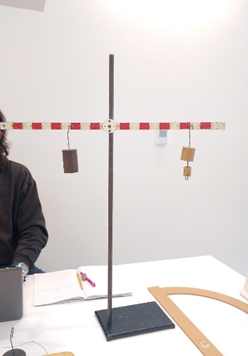
\includegraphics[width=0.3\textwidth]{Imágenes, tablas y gráficas/montaje1.png} 
    \label{fig:Mon1}
\end{figure}
\bigskip
\\La segunda imagen presenta el montaje en el que se utiliza el transportador para medir el ángulo de inclinación de la barra, mientras que se varían los pesos en ambos lados de la barra de equilibrio.
\bigskip
\begin{figure}[ht]
    \centering
    \caption{Montaje con la barra en posición horizontal}
    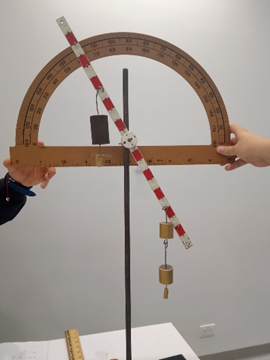
\includegraphics[width=0.3\textwidth]{Imágenes, tablas y gráficas/montaje2.png} 
    \label{fig:Mon2}
\end{figure}
\bigskip

\section*{Metodología}
Primero, se ubicó una masa para tener como referencia a un lado del eje de rotación de la barra. Así, solo se cambiarían las masas y sus respectivas distancias al otro lado del eje. Después, se ubicaron distintas masas buscando que la barra permaneciera horizontal y, con ello, que el sistema permaneciera en equilibrio. Este ejercicio se realizó en cinco ocasiones. Los datos se registraron en una tabla y, con la información en unidades del Sistema Internacional, se hicieron los cálculos respectivos y se construyó una gráfica que relacionara el peso y la distancia de cada masa. 


\section*{Datos, cálculos y gráficas}
A un lado del eje de rotación se dispuso un punto de referencia, es decir, una masa fija a una distancia que no cambió durante la práctica. La masa era de 250 gramos y estaba a una distancia de 20 centímetros. Al convertir tales datos a las unidades correspondientes al Sistema Internacional, se tiene que la masa de referencia era de \( m_{\text{ref}} = 0.25 \, \text{kg} \) y, con ello, el peso era de \( \vec{W}_{\text{ref}} = 2.45 \, \text{N} \); su distancia con respecto al eje de rotación era de \( x_{\text{ref}} = 0.2 \, \text{m} \). En este orden de ideas, la relación matemática entre las masas y las distancias que sí variaban debe corresponderse a la siguiente ecuación:
\[
\vec{W}_{\text{ref}} \cdot x_{\text{ref}} = \vec{W}_{\text{var}} \cdot x_{\text{var}}
\]
Al reemplazar \( \vec{W}_{\text{ref}} = 2.45 \, \text{N} \) y \( x_{\text{ref}} = 0.2 \, \text{m} \) por sus valores numéricos, se tiene:
\[
2.45 \cdot 0.2 = 0.49 = \vec{W}_{\text{var}} \cdot x_{\text{var}}
\]
Así, al momento de comparar la relación de los datos obtenidos a través de las herramientas de Microsoft Excel para graficar será 
\[
\vec{W}_{\text{var}} = \frac{0.49}{x_{\text{var}}}
\]
Dejando un lado fijo –con los datos mencionados previamente–, se ubicaron diferentes masas a diversas distancias al lado contrario del eje de rotación. Todo esto buscando que la barra de equilibrio quede en posición horizontal. Los datos obtenidos en esta primera parte de la práctica de laboratorio se presentan en el cuadro 1:

\bigskip

\renewcommand{\arraystretch}{1.5}
\begin{table}[h]
    \centering
    \caption{Cálculo del peso al otro lado del eje de rotación en cada inteno}
    \begin{tabular}{|>{\centering\arraybackslash}p{1.5cm}|>{\centering\arraybackslash}p{1.5cm}|>{\centering\arraybackslash}p{1.5cm}|>{\centering\arraybackslash}p{1.5cm}|>{\centering\arraybackslash}p{1.5cm}|>{\centering\arraybackslash}p{1.5cm}|}
        \hline
        Intento & \textit{x} (cm) & \textit{x} (m) & \textit{m} (g) & \textit{m} (kg) & \textit{\( \vec{W} \)} (N) \\
        \hline
        1 & 2.5	& 0.025 & 2000 & 2 & 19.60 \\
        \hline
        2 & 5 & 0.05 & 1000 & 1 & 9.80 \\
        \hline
        3 & 10 & 0.1 & 500 & 0.5 & 4.90 \\
        \hline
        4 & 12.5 & 0.125 & 400 & 0.4 & 3.92 \\
        \hline
        5 & 25 & 0.25 & 200 & 0.2 & 1.96 \\
        \hline
    \end{tabular}
\end{table}

\bigskip

A partir de estos datos se construyó la gráfica expuesta en la figura \ref{fig:Graf}, tomando como variable independiente la distancia de la masa con respecto al eje de rotación y como variable dependiente el peso de cada una de las masas. 
\bigskip

% Añadiendo la gráfica
\begin{figure}[ht]
    \centering
    \caption{Relación entre la distancia de la masa y el peso de la misma}
    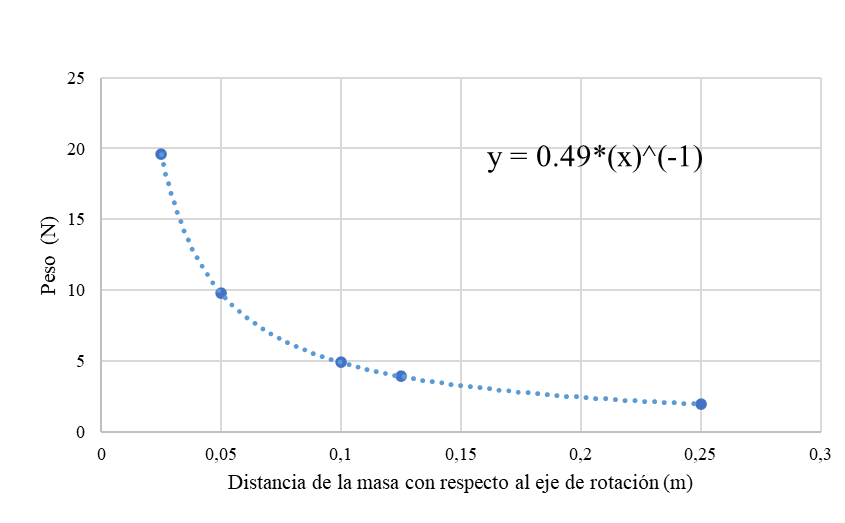
\includegraphics[width=0.8\textwidth]{Imágenes, tablas y gráficas/Gráfica1.png} 
    \label{fig:Graf}
\end{figure}
\bigskip

A través de la regresión de potencias, se obtuvo que la relación matemática era \( y = \frac{0.49}{x} \). Así pues, parece que hay identidad entre la ecuación expuesta en la gráfica y la ecuación obtenida a través de los cálculos expuestos al inicio de la sección:
\[
y = \frac{0.49}{x} \quad \Leftrightarrow \quad \vec{W}_{\text{var}} = \frac{0.49}{x_{\text{var}}}
\]
Así las cosas, es posible calcular el error relativo:
\[
\text{Err}_{\text{rel}} = \frac{|0.49 - 0.49|}{0.49} \times 100\% = 0\%
\]

\section*{Análisis}


\section*{Conclusiones}



\bibliography{Bibliografía/Referencias}

\end{document}
